% * How many of original goals were achieved? Proved to have been achieved
% * Did the program really work?
% *! Credit for interesting conclusion

% ************
% Should have: 
% 	intro
% 	content
% 	summary
% ************

% What I want to say
%
% Questions to answer:
% * Are Distributed Hash Tables viable data stores for a distributed search engine?
% * Do they scale with size?
% * How do Chord and Pastry compare?
%
% Discuss how started with factorial design with factors of nodes and rate.
% Found doesn't vary over length of run, so any run viable.
% All data from three separate runs.
%
% What looked at was latency and success rate.
% 
% Findings to comment on:
% * Why is Chord so much slower than Pastry?
% * Why does Chord has such a low yield rate compared to Pastry
%
% Conclude
% * Does it work for search engine?

\section{Evaluation}
In this chapter I will look at how the performance of Chord and Pastry compare. I will also briefly discuss the benefits of the proximity heuristic used in routing by Pastry, and finally I will discuss if Distributed Hash Tables are good back end stores for a distributed search engine of the kind I have built.

\subsection{What to evaluate}
% Questions to answer:
% * Are Distributed Hash Tables viable data stores for a distributed search engine?
% * Do they scale with size?
% * How do Chord and Pastry compare?
% What looked at was latency and success rate.
I will take a quantitative approach when evaluation the Distributed Hash Tables Chord and Pastry. What interests me is if they could work well as data stores in the distributed friend search engine I have built. To that extent what I will be evaluating is the latency and success rate of key lookups in the network.

We will also look at how the performance is affected by the size of the Distributed Hash Table network, and pit Chord against Pastry to see which one performs best.

\subsection{Experimental design}
% Discuss how started with factorial design with factors of nodes and rate.
% Found doesn't vary over length of run, so any run viable.
% All data from three separate runs.
I ran my Distributed Hash Tables on machines in the Planet-Lab network. With that in mind, the variables I was able to control were the number of machines participating in the system, the number of Distributed Hash Table nodes running on each machine, and the rate of requests in the network.

In my tests I used all the machines available to me to give some scale to the experiments, and limited the experimental factors to the number of nodes run on each machine and the rate at which requests were issued.

My experiments follow a factorial design where both node count and rate varied between 1 and 16 in powers of two. Each configuration was run at three different occasions for both Chord and Pastry. The combined log files for each experimental configuration were then used to give the results I am about to present.

\subsubsection{Experimental pattern}
Each experimental run followed a predefined pattern:
\begin{enumerate}
\item I would ensure that the correct number of nodes was running
\item If the number of nodes had to be adjusted, the nodes would be given 3 minutes to update their routing tables.
\item Each machine would clear its previous logs and start its logging machinery.
\item After that the actual experiment would start. Each machine would issue requests to the nodes it hosted at a rate specified for that particular experimental run.
\item After a successfully completed run, there would be a cool down period with continued logging where requests taking slightly longer than permitted would be allowed to finish. Logging would then stop and the logs from the individual machines would be collected at the central hub node.
\item The logs were then downloaded from the central hub to my personal machine for safekeeping and analysis.
\item The process was then repeated for different experimental parameters.
\end{enumerate}

\subsection{Effects of Planet-Lab}
As previously mentioned my experiments ran on top of machines provided by Planet-Lab. I was allowed to run up to 100 machines, but never managed to get quite that many up and running at the same time.

Using Planet-Lab as a test bed gave me several benefits: the machines at my disposal had a high geographical spread, and varied greatly in what computational resources they provided. Depending on the time of day the computational load on the machines would also vary and not only that, but I would have a different subset of the machines available for testing from day to day.

This provided an excellent foundation for testing Distributed Hash Tables which are meant to be able to cope with high node churn and machines with widely different capabilities.

While Planet-Lab provides an interesting test bed, the randomness with which computational resources are available makes it impossible to accurately repeat experiments. Rerunning an experiment would invariably give a slightly different result.
To work with Planet-Lab's strengths and not against it, and at the same time to get data I could have confidence in, I ran each experiment multiple times, shifted in time. This way I ensured I would sample different subsets of the topology. I believe this gave me results that while having higher variance, also more closely resemble the real world scenario Distributed Hash Tables are likely to find themselves in.

\subsubsection{Experimental cleanliness and validity of results}
Performing experiments over longer periods of time showed that the success rate (figure \ref{figLatencyAgainstTime}) and latency (figure \ref{figRateAgainstTime}) for all practical purposes stay constant over time. This allowed me to cut down the length of individual experimental runs without lowering the quality of my results.

\begin{figure}[!htb]
  \begin{center}
    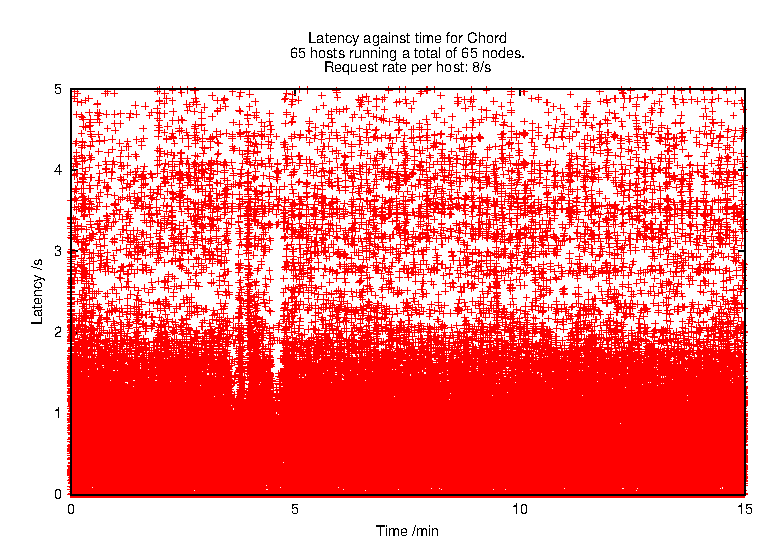
\includegraphics[]{illustrations/latency_aginst_time_chord.eps}
    \caption{This graph shows how latency vary with time in a 15 minute experimental run of Chord.}
    \label{figLatencyAgainstTime}
  \end{center}
\end{figure}

\begin{figure}[!htb]
  \begin{center}
    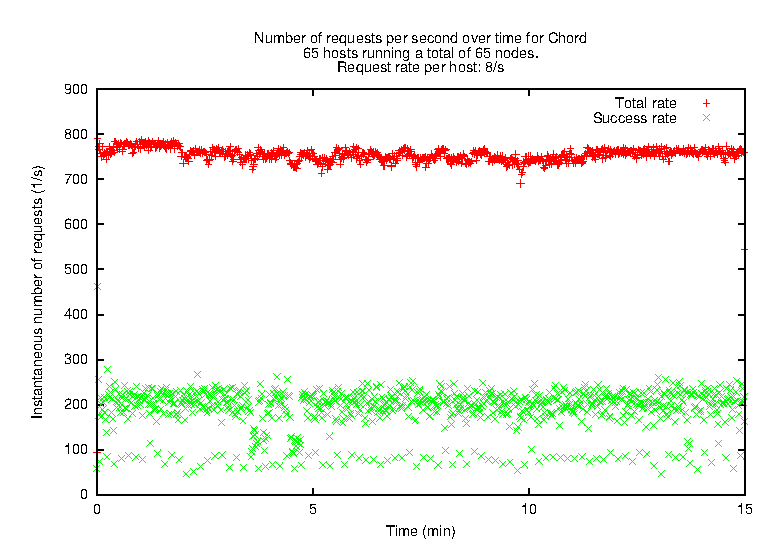
\includegraphics[]{illustrations/rate_against_time_chord.eps}
    \caption{This graph shows how the request rate and success rate varies over a 15 minute experimental run of Chord.}
    \label{figRateAgainstTime}
  \end{center}
\end{figure}

% * How logging not affect results
During experimental runs I would turn of all functionality not directly needed for serving the requests. This would include turning of the mechanisms that kept the nodes routing tables up to date. If a node disappeared during an experiment, nodes contacting it directly would take note of it, but other nodes wouldn't have the nodes disappearance reflected in their routing state like they would under normal operation. This might seem a somewhat unnatural choice, but makes sense for my experiments for the following reasons:

In my experimental builds of Chord and Pastry I had turned up the rate a which routing information was dissipated through the network to an extreme to cut down the waiting time between experimental runs. Since what I wanted to test was the raw performance of the system, removing the overhead of keeping the routing tables up to date made sense, since this overhead differs between Chord and Pastry, and is a parameter that would have to be tweaked before using this system in any real world deployment.
Also having established that the length of the experimental runs was insignificant made me confident in that not updating routing information during experimental runs did no harm to the experimental results.

% * How load spread evenly
\mbox{}
To ensure even load across my test network, each machine involved individually issued requests to the Distributed Hash Table network.
The keys looked up were randomly generated by hashing a combination of the Ip-address of the machine issuing the request and a time stamp. This approach results in keys that differ from experimental run to experimental run. While this makes doing repeatable experiments impossible, it nicely models a real world spread of keys that otherwise would be hard to predict and also evenly spreads the loads between the machines.

% * What constitutes a valid run
Data from experimental runs where a significant number of machines disappeared during the run would be discarded.


\subsection{Results}
Throughout my experiments, a valid request is defined as a request that completes within 5 seconds. By that definition, all other requests are invalid, regardless of if they fail to complete at all, or if they just complete after more than 5 seconds have passed.
% Comment on what is a valid request. And what is considered a failed request
% Findings to comment on:

\subsubsection{Mean latency and success rate for Chord and Pastry}
In figure \ref{figChordLatency} and \ref{figPastryLatency} you see the latency for different rates and different number of nodes per machine for around 60 machines, shown with 95\% confidence intervals. 

What is immediately noticeable is how much more variance there is in the latencies for Chord than there is in the latencies for Pastry.
In the case of Pastry (figure \ref{figPastryLatency}) we see how the latencies consistently grow for larger number of nodes. Intuitively this is what we would expect as the theory behind the Distributed Hash Tables tells us the number of nodes involved in a look up is proportional to the logarithm of the number of nodes in the network and the higher the number of nodes, the more the inter-node connectivity latency plays a role. The same trend is not apparent for Chord (figure \ref{figChordLatency}). On the contrary there is no apparent correlation between the number of nodes and the latency for a given rate. What is also peculiar in the Chord dataset is that, looking at the latencies for a fixed number of nodes per host, the latencies seem to decrease for higher loads.

\begin{figure}[!htb]
  \centering
  \subfigure[Latency for Chord]{
    \label{figChordLatency}
    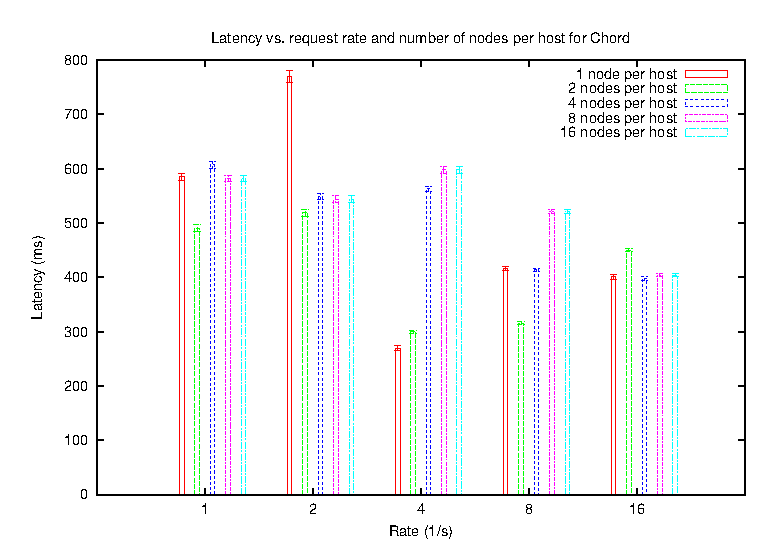
\includegraphics[]{illustrations/latency_chord.eps}
  }
  \subfigure[Latency for Pastry]{
    \label{figPastryLatency}
    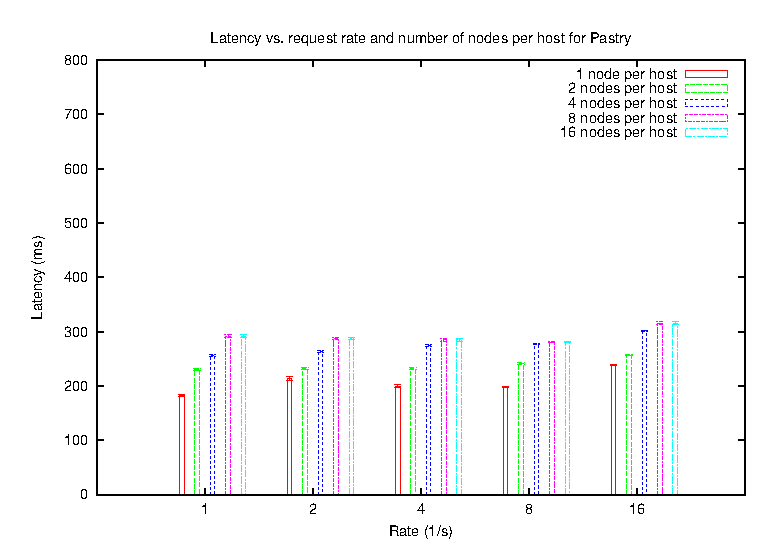
\includegraphics[]{illustrations/latency_pastry.eps}
  }
  \caption{These graphs show the latencies for (a) Chord and (b) Pastry with 95\% confidence intervals for set-ups of slightly above 60 nodes.}
\end{figure}

\begin{figure}[!htb]
  \centering
  \subfigure[Success rate for Pastry]{
    \label{figPastrySuccessRate}
    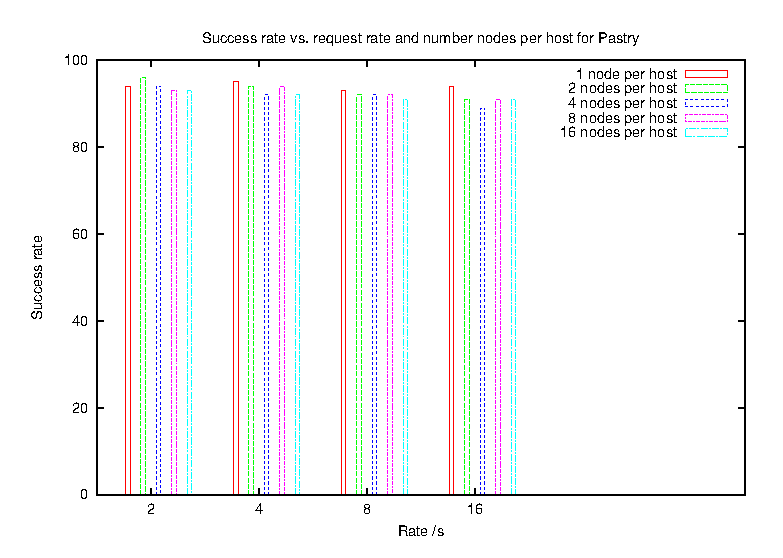
\includegraphics[]{illustrations/success_rate_pastry.eps}
  }
  \subfigure[Success rate for Chord]{
    \label{figChordSuccessRate}
    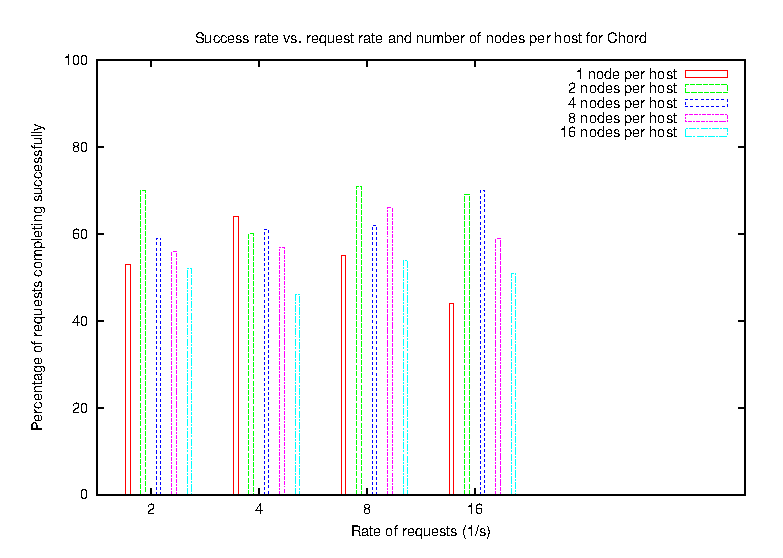
\includegraphics[]{illustrations/success_rate_chord.eps}
  }
  \caption{These graphs show the instantaneous rate of request and the instantaneous rate of successfully completed requests sampled once per second for (a) Chord and (b) Pastry. In each case with experimental set-ups of slightly above 60 nodes.}
\end{figure}

The success rate is also dramatically different between Chord (figure \ref{figChordSuccessRate}) and Pastry (\ref{figPastrySuccessRate}). Chord seems to perform better when more than one node is run on the same machine, while Pastry's success rate slightly decreases the more nodes are run on the same physical hardware. It is also worth noting that even at its best, Chord can't compare with the worst case performance of Pastry.

Unfortunately I have no good explanation for the variations we see within the different configurations for Chord, but I can explain why Chord in the general performs so much worse than Pastry, and I will do so shortly.

Before that I want to discuss how Chord and Pastry behave when pushed to their limits. The cumulative distribution functions for Chord (figure \ref{figChordCDF}) and Pastry (figure \ref{figPastryCDF}) show the percentage of requests that succeed within five seconds. The experiments are run on roughly 60 machines hosting 1 node each. We see how the success rate gracefully drops for extreme rates with Pastry.
In the case of Chord on the other hand, the success rate is only marginally worse for 128 and 64 requests per second per hosts than when there are 16 requests per second per machine. Also rather odd is how the rate of 2 requests per second performs significantly worse than what does the rate of 4 in the case of Chord. I have no good explanations for this behaviour.

Please also notice how the cumulative distribution function graph seems to plateau relatively quickly after around twice the average latency. What this seems to tell us is that if a request does not succeed within a relative short window of time, the probability of it still returning successfully is vanishingly small. This knowledge could be used to set sensible time-out values for lookups.

\begin{figure}[!htb]
  \centering
  \subfigure[Cumulative distribution function of success against latency for Chord]{
    \label{figChordCDF}
    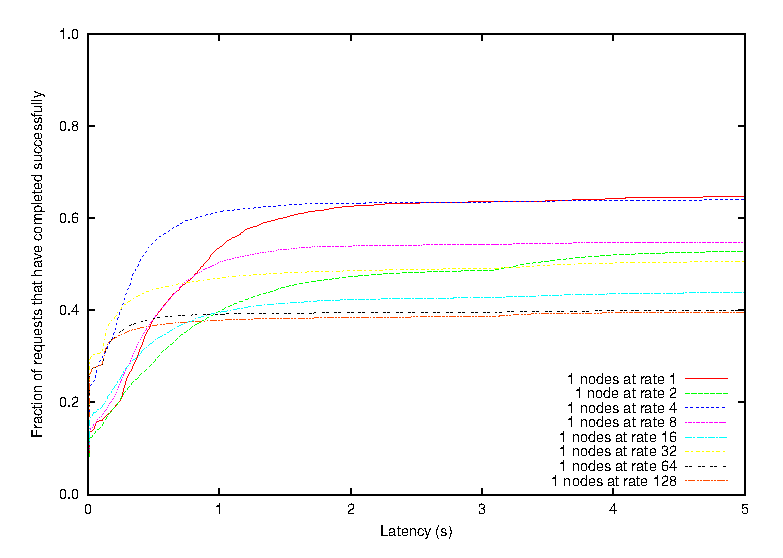
\includegraphics[]{illustrations/cdf_chord.eps}
  }
  \subfigure[Cumulative distribution function of success against latency for Pastry]{
    \label{figPastryCDF}
    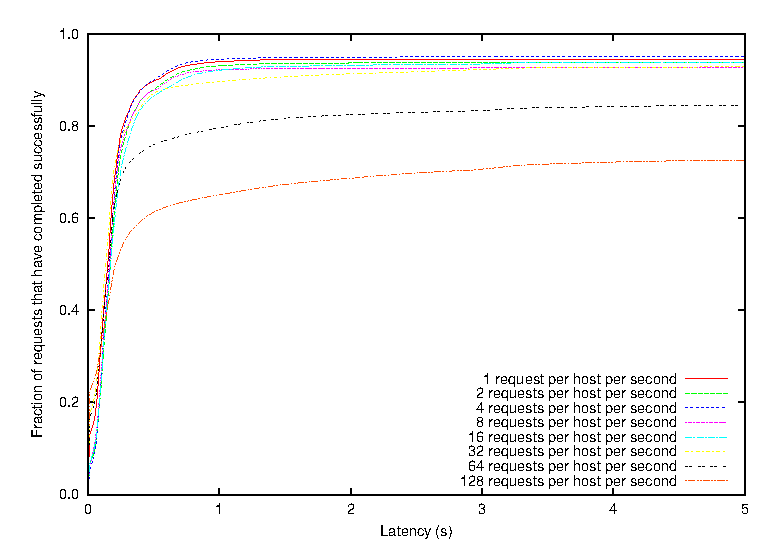
\includegraphics[]{illustrations/cdf_pastry.eps}
  }
  \caption{The graphs above show the cumulative distribution function of a request being successful within the first 5 seconds for (a) Chord, and (b) Pastry.}
\end{figure}

\subsubsection{Why Chord performs worse that Pastry}
The experimental evidence shown so far shows Pastry as superior to Chord both in terms of latency and in the success rate of requests. I will now try to explain in turn what the causes might be.

\mbox{}

The higher latencies of Chord are the easiest to explain. In figure \ref{figChordNumNodes} and \ref{figPastryNumNodes} you see how many nodes are involved in key lookups for Chord and Pastry respectively. It is clear from the graph that the average number of nodes involved in a key lookup are greater for Chord than for Pastry. If one multiplies the average time it takes two randomly chosen nodes to connect with the number of nodes involved in a key lookup, it should be clear that a Chord lookup should take longer if the only thing one is accounting for is the latency of the routing. We are also not factoring in that Pastry uses a heuristic when routing, favouring nodes closer by, which also affects the latency as each routing step is likely to take less time for Pastry than it does for Chord. I will shortly discuss the impact of the proximity heuristic in Pastry.

Whether the higher number of routing steps for Chord is a bug introduced by me or something inherent to the Chord algorithm is something I can't comment on. It is also possible that the difference would become less significant for larger networks of nodes. Unfortunately this is not something I was able to test given the infrastructure available to me.

\begin{figure}[!htb]
  \centering
  \subfigure[Number of nodes involved in key lookup for Chord]{
    \label{figChordNumNodes}
    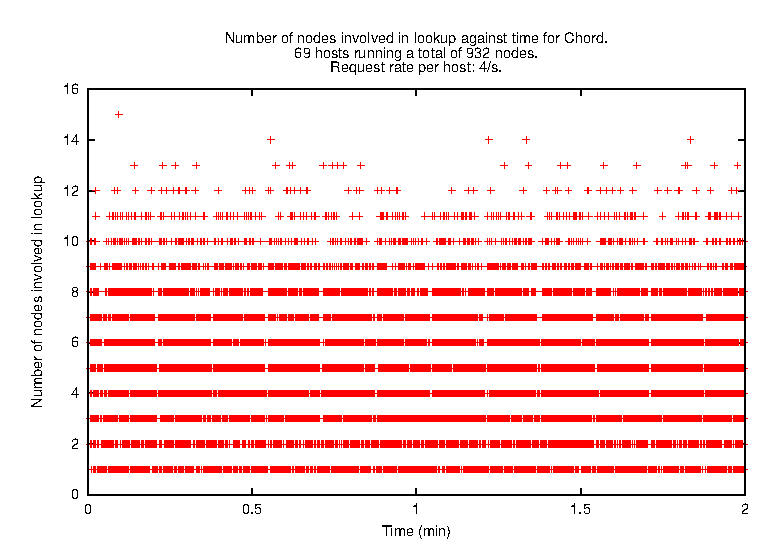
\includegraphics[]{illustrations/nodes_against_time_chord.eps}
  }
  \subfigure[Number of nodes involved in key lookup for Pastry]{
    \label{figPastryNumNodes}
    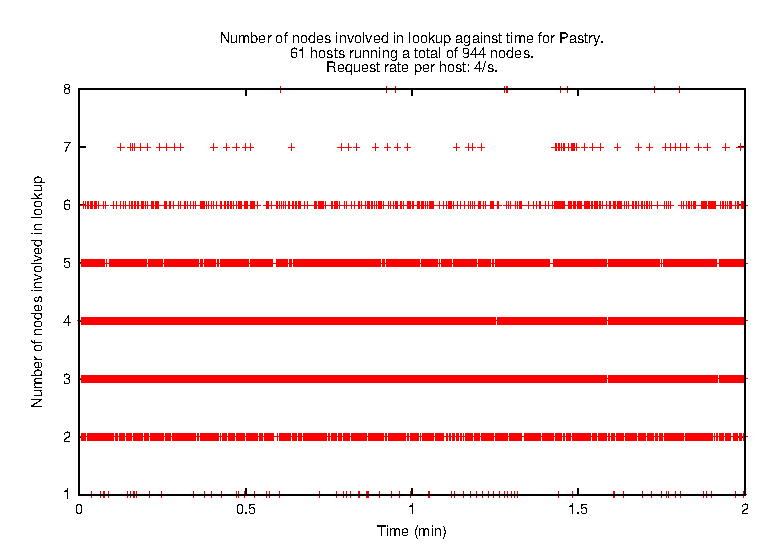
\includegraphics[]{illustrations/nodes_against_time_pastry.eps}
  }
  \caption{The graphs show the number of nodes involved in a key lookup for (a) Chord and (b) Pastry for a particular experimental run.}
\end{figure}

\mbox{}
Now that we have an idea of why the latency might be higher for Chord than for Pastry, let me try to explain why the failure rate is higher as well.

First let us recall how Chord and Pastry perform their routing.
In Chord, the node that wants to lookup a key (the requester) asks the node closest to the key that it knows about if it knows about other nodes closer to the target key. It then asks the node it gets returned the same question, and the pattern continues until it finds the node immediately preceding the key. Its successor is the target node responsible for the key.

Pastry follows a different approach. When a requesting node looks up a key it makes a request to the node it knows about that is closest to the target node. Where it differs from the Chord approach is that the requester hands over the responsibility for the continued lookup to the node it asked. This node in turns then asks another node until the target node has been reached.

Now lets consider what happens when something goes wrong.
In figure \ref{figChordFailedLookup} we see what happens when Chord node A gets returned node D as the next hop node from B. D is not accessible and the lookup fails. If A retries the routing step, B again returns D, unless it in the meantime itself has noticed that D is inaccessible.

In the case of Pastry node B becomes responsible for routing the request forward towards the target node. Upon realising node D is unavailable it routes it to the next closest node it knows about, in this case C. Node C happens to know about a node closer to the target than B does and this way we managed to route around the unavailable node D.

There are workarounds for improving Chord's routing performance. One would be for the requesting node A to inform node B about node D's death upon retrying to route the message. An alternative could also have been for A to try to route the request through another intermediate node before D, but in this case we are not guaranteed that this intermediate node will not also return D.
A third approach could be to look up D's predecessor, and then use that node in the same role previously filled by B. None of these methods have been used in my implementation as they would extend the core Chord routing algorithm and therefore skew the comparison in Chord's favour.

\begin{figure}[!htb]
  \centering
  \subfigure[Failed lookup in Chord]{
    \label{figChordFailedLookup}
    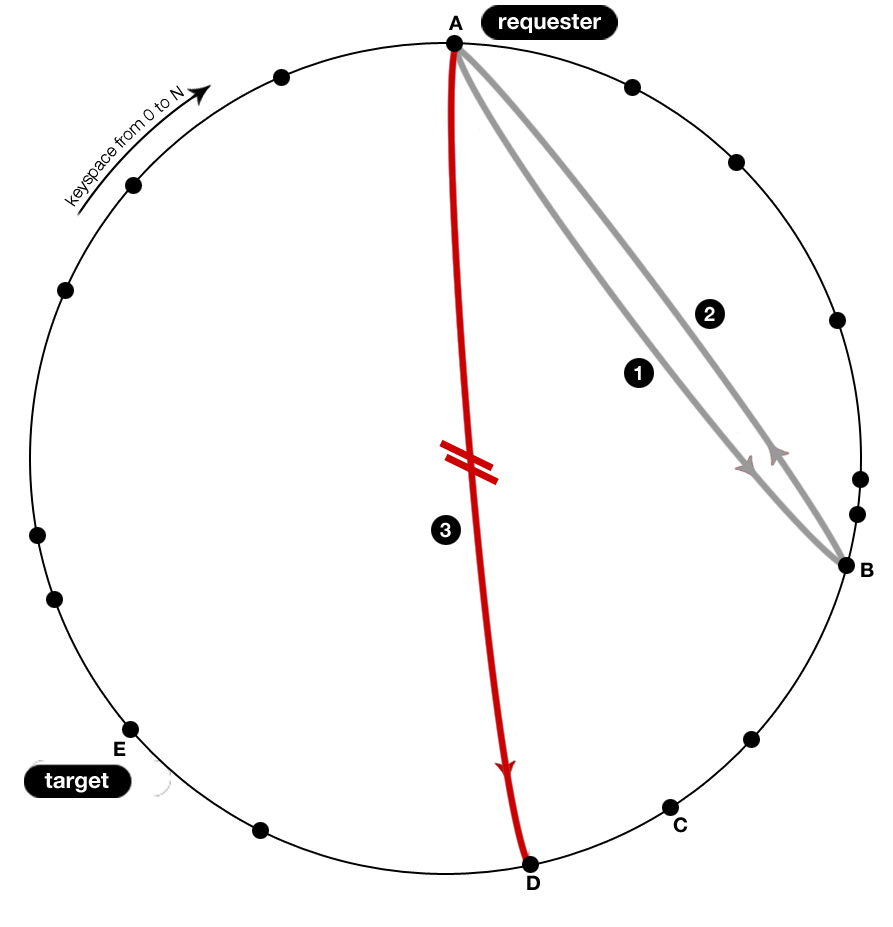
\includegraphics[]{illustrations/ChordRoutingFailed.png}
  }
  \subfigure[Failed lookup in Pastry]{
    \label{figPastryFailedLookip}
    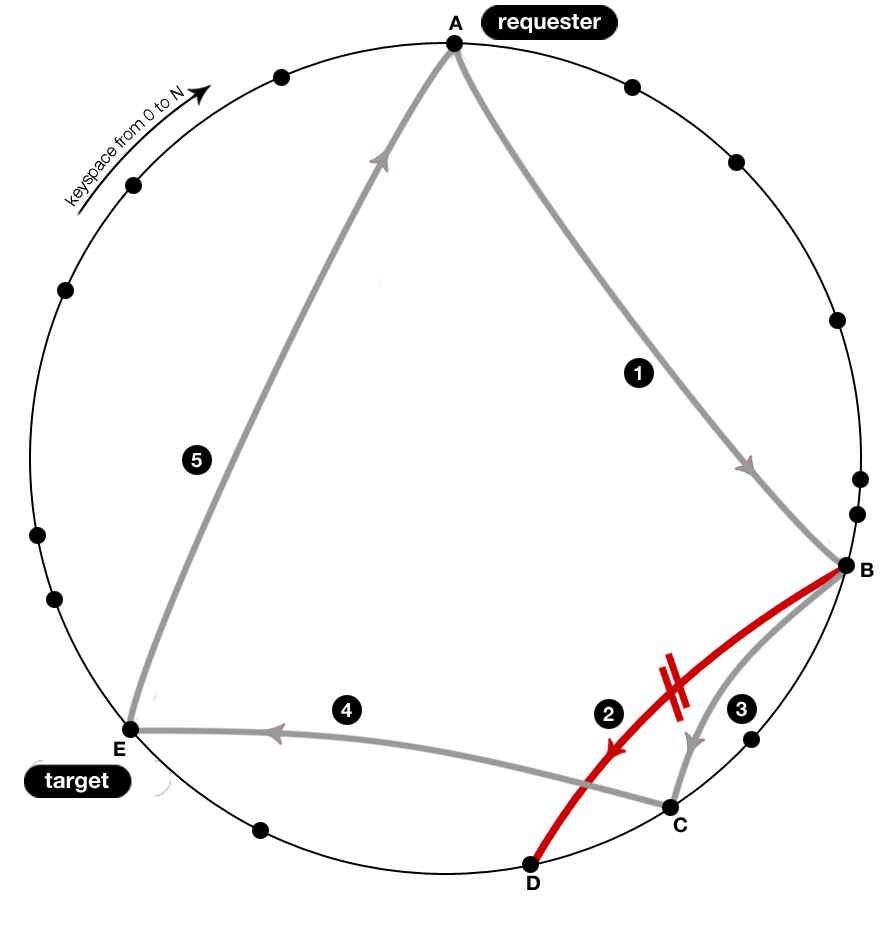
\includegraphics[]{illustrations/PastryRoutingFailed.png}
  }
  \caption{The illustrations show the differences in the routing approach of Chord and Pastry in the case where one of the nodes in the lookup chain is not accessible (Node D). In the case of Pastry it routes around the failed node, while Chord if trying to route again will again get node D returned by node B.}
\end{figure}

% * Why is Chord so much slower than Pastry?
% * Why does Chord has such a low yield rate compared to Pastry
% * How much can we conclude from the numbers?

\subsection{Effect of Pastry routing heuristics}
% * What effect does the Pastry routing heuristics have on the performance
In this section I will look at how the heuristics used in my implementation of Pastry affect the routing performance. 

I have sampled the latencies from Pastry in a small set of different configurations with the heuristic enabled and then with the heuristic turned off. Please note that this is nothing but a very limited sample and by no means an exhaustive evaluation of the heuristic, or heuristics in general. One should not try to generalize the findings based on this data or read it as valid for anything but the sampled configurations.

The following configurations were sampled:
\begin{itemize}
\item 10 machines running 1 node each
\item 10 machines running 5 nodes each
\item 50 machines running 1 node each
\item 50 machines running 16 nodes each
\end{itemize}

The choice of configurations were made for the following reason:
I wanted to see how expanding the network by adding additional machines at new geographical locations affect the latency.
I also wanted to see how running 50 nodes across a few machines compared to running 50 nodes on 50 different machines. Lastly I also wanted to see how the heuristic behaved in the more extreme case with a larger network with relatively large cliques of nodes close to each other.

The results seen in figure \ref{figPastryHeuristic} partly show what one would expect, in other words that the heuristic improves the routing performance.

\begin{figure}[!htb]
  \begin{center}
    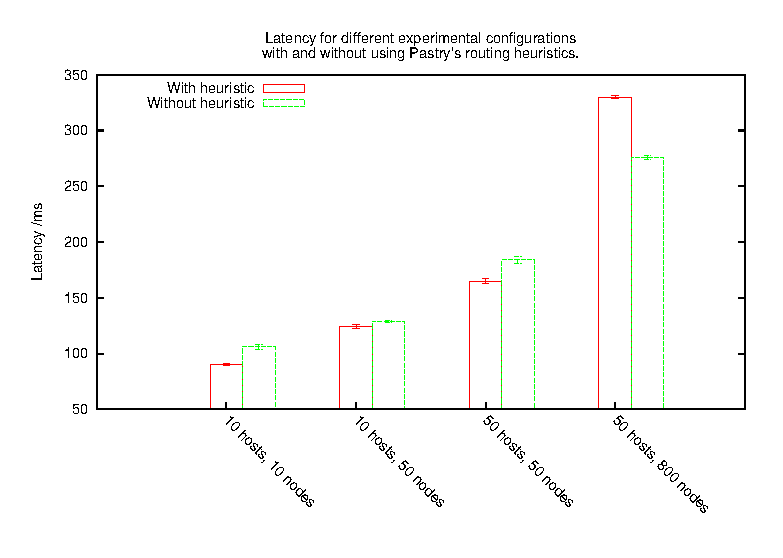
\includegraphics[]{illustrations/pastry_heuristic.eps}
    \caption{Latencies for Pastry with and without the routing proximity heuristic activated. Shown with 95\% confidence intervals.}
    \label{figPastryHeuristic}
  \end{center}
\end{figure}

As one would expect, the heuristic allowing nodes to preferentially route to geographically closer nodes for the most part improved the performance substantially. In the two cases where only 1 node were run per host we see a 15\% and 10\% gain for the 10 machine and 50 machine cases respectively.
Quite surprisingly, the cases where multiple nodes are located on the same machine, a scenario where I would have expected the heuristic to shine, perform less well. In the case where 50 nodes are spread over 10 hosts we only see a 4\% performance gain when using the heuristic, and in the case where 50 machines run 16 nodes each, the performance drops by 20\% when the heuristic is being used.

Unfortunately I have no conclusive evidence indicating what could cause the performance drop when there are many nodes running on the same machine. The heuristic is only calculated when nodes are added to the routing table, and should therefore not affect the routing performance locally within a node.

Maybe the heuristic of hop count in the underlying network is just suboptimal.

Nothing much can be concluded from this, other than that heuristics do not necessarily result in performance gains unless chosen carefully. This outcome also highlights the importance of relying on metrics when making design decisions rather than blindly implementing performance enhancements in the faith that optimisations are always for the better.

Less interesting, but reassuring non the less, is that the latency grows with increasing number of nodes in the network, just like one would expect. Unfortunately this dataset does not allow for a general measure of how the latency grows with the network size.

\subsection{Viability of Chord and Pastry as back end data stores for a search engine}
% Conclude
% * Does it work for search engine?
In its current raw form, Chord is not really a viable data store for any application. Its high and variable latency, although undesirable, is something one could live with, if the key lookups would not have such a high failure rate.

Pastry on the other hand proves a quite efficient key value data store, even in highly distributed environments. Its combination of high success rates and consistently low key lookup latencies and gradual degradation in performance under high load are all desirable properties.

I would have to say that using key-value stores as back end data stores for a search engine is only a good solution if you can combine ways of getting the data evenly spread in the key-space with ways of easily querying it.
A slightly optimized version of the link record system proposed in this dissertation can work for small to medium scale installations, but unfortunately it doesn't seem to scale well enough for larger implementations unless link records are aggressively cached at the end systems.

\mbox{}

In this chapter we have seen how my implementation of Pastry outperforms my implementation of Chord both in terms of latency and key lookup success rate.
We have also discovered how the proximity heuristic used in routing by Pastry quite counter intuitively does not always yield performance improvements, and have understood the importance of relying on metrics rather than intuition when evaluating system performance.

Finally we concluded that for small to medium scale search engines of the type proposed in this dissertation, using a distributed hash table as the back end data store might work reasonably well, and that caching link records at end the end systems might be used to increase performance.
